\documentclass[11pt, a4paper]{report}

% --- Packages ---
\usepackage[utf8]{inputenc}
\usepackage[T1]{fontenc}
\usepackage{lmodern}
\usepackage{geometry}
\geometry{a4paper, margin=1in}
\usepackage{amsmath, amssymb, amsfonts}
\usepackage{booktabs}
\usepackage{float}
\usepackage{graphicx}
\usepackage{hyperref}
\usepackage{caption}
\usepackage{array}
\usepackage{titlesec}
\usepackage{tabularx}
\usepackage{ragged2e}
\usepackage[table]{xcolor}
\usepackage{parskip}

% --- Document Info ---
\titleformat{\chapter}[hang]{\huge\bfseries}{\thechapter.\ }{0pt}{\huge\bfseries}
\titlespacing*{\chapter}{0pt}{-20pt}{20pt}
\title{Event-Based Vision and State Space Models for Object Detection and Autonomous Obstacle Avoidance on Micro UAVs}
\author{Benas Vaiciulis}
\date{March 2026}

\begin{document}

% --- Title Page ---
\begin{titlepage}
    \centering
    \vspace*{1cm}
    \Large\textbf{Event-Based Vision and State Space Models for Object Detection and Autonomous Obstacle Avoidance on Micro UAVs} \\
    \vspace{0.5cm}
    \large Thesis A Interim Report and Project Plan \\
    \vspace{1.5cm}
    \textbf{Author:} Benas Vaiciulis \\
    \textbf{Supervisor:} Will Midgley\\
    \vspace{1.5cm}
    UNSW Sydney \\
    School of Mechanical and Manufacturing Engineering \\
    \vfill
    March 2026
\end{titlepage}

% --- Abstract ---
\begin{abstract}
This report presents a thesis investigating State Space Models (SSMs) for real-time object detection and autonomous obstacle avoidance on micro UAVs using event-based camera data. Event-based cameras offer microsecond temporal resolution and high dynamic range, making them well-suited for agile UAV perception. Existing architectures fail to exploit the asynchronous nature of event streams, while transformer-based methods impose prohibitive computational cost. SSMs provide linear-time sequence modelling with significantly less performance degradation than RNN or transformer-based approaches across variable event rates. The S5-RVT baseline was successfully reproduced at 47.7~mAP@0.5 on the Gen1 dataset, confirming the evaluation pipeline. Literature review, research plan, and preliminary results are presented.
\end{abstract}

\tableofcontents

% --- Nomenclature ---
\chapter*{Nomenclature}
\addcontentsline{toc}{chapter}{Nomenclature}
\begin{tabular}{ll}
\multicolumn{2}{l}{\textit{Latin Symbols}} \\[4pt]
$A$ & state transition matrix \\
$\bar{A}$ & discretised state matrix \\
$B$ & input projection matrix \\
$\bar{B}$ & discretised input matrix \\
$C$ & contrast threshold \\
$C_{ssm}$ & SSM output projection matrix \\
$d_{model}$ & model embedding dimension \\
$h(t)$ & hidden state vector (continuous time) \\
$h(k)$ & latent state vector at discrete step $k$ \\
$L(x,y,t)$ & log luminance \\
$P$ & event polarity (+1 or -1) \\
$I$ & identity matrix \\
$t$ & time, s \\
$u(t)$ & input signal \\
$x, y$ & pixel coordinates \\[8pt]
\multicolumn{2}{l}{\textit{Greek Symbols}} \\[4pt]
$\Delta$, $\Delta t$ & SSM discretisation step size (used interchangeably) \\[8pt]
\multicolumn{2}{l}{\textit{Acronyms}} \\[4pt]
CNN & Convolutional Neural Network \\
DAVIS & Dynamic and Active-pixel Vision Sensor \\
DVS & Dynamic Vision Sensor \\
EST & Event Spike Tensor \\
GNN & Graph Neural Network \\
HDR & High Dynamic Range \\
LIF & Leaky Integrate-and-Fire \\
LTI & Linear Time-Invariant \\
RNN & Recurrent Neural Network \\
SNN & Spiking Neural Network \\
SSM & State Space Model \\
SSD & Single Shot MultiBox Detector \\
SWaP & Size, Weight, and Power \\
UAV & Unmanned Aerial Vehicle \\
\end{tabular}

% --- Chapter 1: Introduction ---
\chapter{Introduction}
Micro unmanned aerial vehicles (UAVs), broadly classified as platforms weighing less than 250 grams, have emerged as transformative tools for applications ranging from infrastructure inspection and search-and-rescue operations to indoor mapping and environmental monitoring \cite{floreano2015science}. Their small form factor enables navigation through confined spaces inaccessible to larger platforms; however, this advantage comes with severe constraints on payload capacity, onboard computational resources, and power budgets. These size, weight, and power (SWaP) limitations represent the central engineering challenge for autonomous micro-UAV systems: the perception and control pipeline must be both highly capable and extremely efficient.

Conventional frame-based cameras, while mature and well-supported by deep learning frameworks, suffer from inherent limitations that are particularly problematic for agile UAV flight. They capture redundant information at fixed frame rates, exhibit motion blur during rapid maneuvers, and possess limited dynamic range. 

Event-based cameras, also known as dynamic vision sensors (DVS), represent a paradigm shift in visual sensing. Unlike frame-based cameras, each pixel in an event camera independently and asynchronously responds to changes in log luminance, generating a stream of events with microsecond temporal resolution, a dynamic range exceeding 120 dB, and minimal motion blur \cite{gallego2020event}. These properties make event cameras inherently suited to the perception requirements of agile micro-UAVs, where rapid obstacle detection and avoidance are critical to safe operation. Several pioneering studies have demonstrated event-based obstacle avoidance on quadrotors \cite{falanga2019fast}, \cite{sanket2020evdodgenet} achieving reaction latencies as low as 3.5 milliseconds. 

Despite these promising sensor characteristics, a significant gap remains in the algorithmic domain. Most existing approaches to processing event data for detection and avoidance rely on converting asynchronous event streams into frame-like representations for consumption by convolutional neural networks (CNNs) or recurrent neural networks (RNNs), thereby discarding much of the temporal richness that distinguishes event cameras from their frame-based counterparts. Transformer-based architectures, while capable of modelling long-range dependencies, impose quadratic computational complexity that renders them impractical for deployment on the severely resource-constrained processors typical of micro-UAVs \cite{vaswani2017attention}. 

State Space Models (SSMs), and in particular the recently developed Mamba architecture and its variants, offer a compelling alternative. SSMs model input sequences through continuous-time linear dynamical systems that can be discretised at arbitrary time steps, achieving linear computational complexity while maintaining strong temporal reasoning capabilities \cite{gu2022efficiently}. Critically, Zubic et al. \cite{zubic2024state} have recently demonstrated that SSMs naturally accommodate the variable temporal resolution inherent to event camera data, enabling deployment at inference frequencies different from training frequencies with significantly less performance degradation than RNN or transformer-based approaches. 

This thesis investigates the integration of state space models with event-based camera data for real-time object detection and autonomous obstacle avoidance on micro-UAVs. The central hypothesis is that SSM-based architectures can more effectively exploit the temporal structure of event streams than existing CNN, RNN, or transformer-based approaches, achieving competitive detection accuracy with reduced computational cost suitable for onboard deployment. The following literature review establishes the relevant foundations and identifies the specific research gaps this work addresses. 

% --- Chapter 2: Literature Review ---
\chapter{Literature Review}

\section{Event-Based Cameras: Principles and Hardware}
Event-based cameras, or neuromorphic vision sensors, operate on a fundamentally different principle from conventional frame-based cameras. Rather than capturing synchronous frames at a fixed rate, each pixel independently monitors changes in log luminance and asynchronously emits an event when the change exceeds a predefined contrast threshold $C$. Formally, a pixel at coordinates $(x, y)$ generates an event $e = (x, y, t, p)$ at time $t$ when $|L(x, y, t) - L(x, y, t - \Delta t)| \geq C$, where $L$ denotes log luminance and $p \in \{+1, -1\}$ indicates the polarity of the brightness change \cite{gallego2020event}, \cite{lichtsteiner2008128x128}. This bio-inspired operating principle, modelled after biological retinal ganglion cells, confers several advantages over frame-based imaging: microsecond temporal resolution (typically 1 µs), very high dynamic range (>120 dB compared to approximately 60 dB for standard cameras), extremely low latency, low power consumption, and the absence of motion blur \cite{gallego2020event}.

Gallego et al. \cite{gallego2020event} provided a comprehensive survey of event-based vision, cataloguing the evolution of neuromorphic sensors from the original silicon retina proposed by Mahowald and Mead in 1992 through to modern commercially available sensors. The Dynamic Vision Sensor (DVS), developed at ETH Zurich, was among the first widely adopted event cameras and demonstrated the feasibility of asynchronous vision for robotics applications \cite{lichtsteiner2008128x128}. A significant advancement came with the Dynamic and Active-pixel Vision Sensor (DAVIS), which combines a DVS with a conventional active pixel sensor on the same die, enabling simultaneous capture of events and intensity frames at the same pixel locations \cite{brandli2014240x180}. The original DAVIS sensor, offering 240×180 pixel resolution, has become a widely used research platform, with later commercial variants such as the DAVIS346 extending this to higher resolutions. 

More recently, Prophesee (formerly Chronocam) has developed a series of commercial event cameras with increasing resolution and performance. The Gen3.1 sensors, used in the DSEC dataset \cite{gehrig2021dsec}, offer VGA-resolution event sensing, while the latest IMX636 sensor, developed in collaboration with Sony, provides 1280×720 HD resolution with ultra-high-speed operation \cite{prophesee2026metavision}. At the opposite end of the spectrum, the GenX320 sensor targets ultra-low-power applications with a 320×320 pixel array consuming as little as 2 mW, making it particularly relevant for resource-constrained micro UAV platforms \cite{prophesee2026metavision}. The continued improvement in sensor resolution, noise characteristics, and power efficiency has been a key enabler for the expanding application of event cameras in robotics and autonomous systems. 

A notable limitation of current event cameras, however, is their relatively low spatial resolution compared to frame-based cameras. While modern frame-based sensors routinely achieve multi-megapixel resolutions, event cameras remain in the VGA to HD range. Furthermore, event cameras produce no output in static scenes, which can be both an advantage (data efficiency) and a limitation (loss of static scene information). These characteristics necessitate careful algorithm design that leverages the temporal strengths of event cameras while mitigating their spatial limitations.

\begin{figure}[ht]
    \centering
    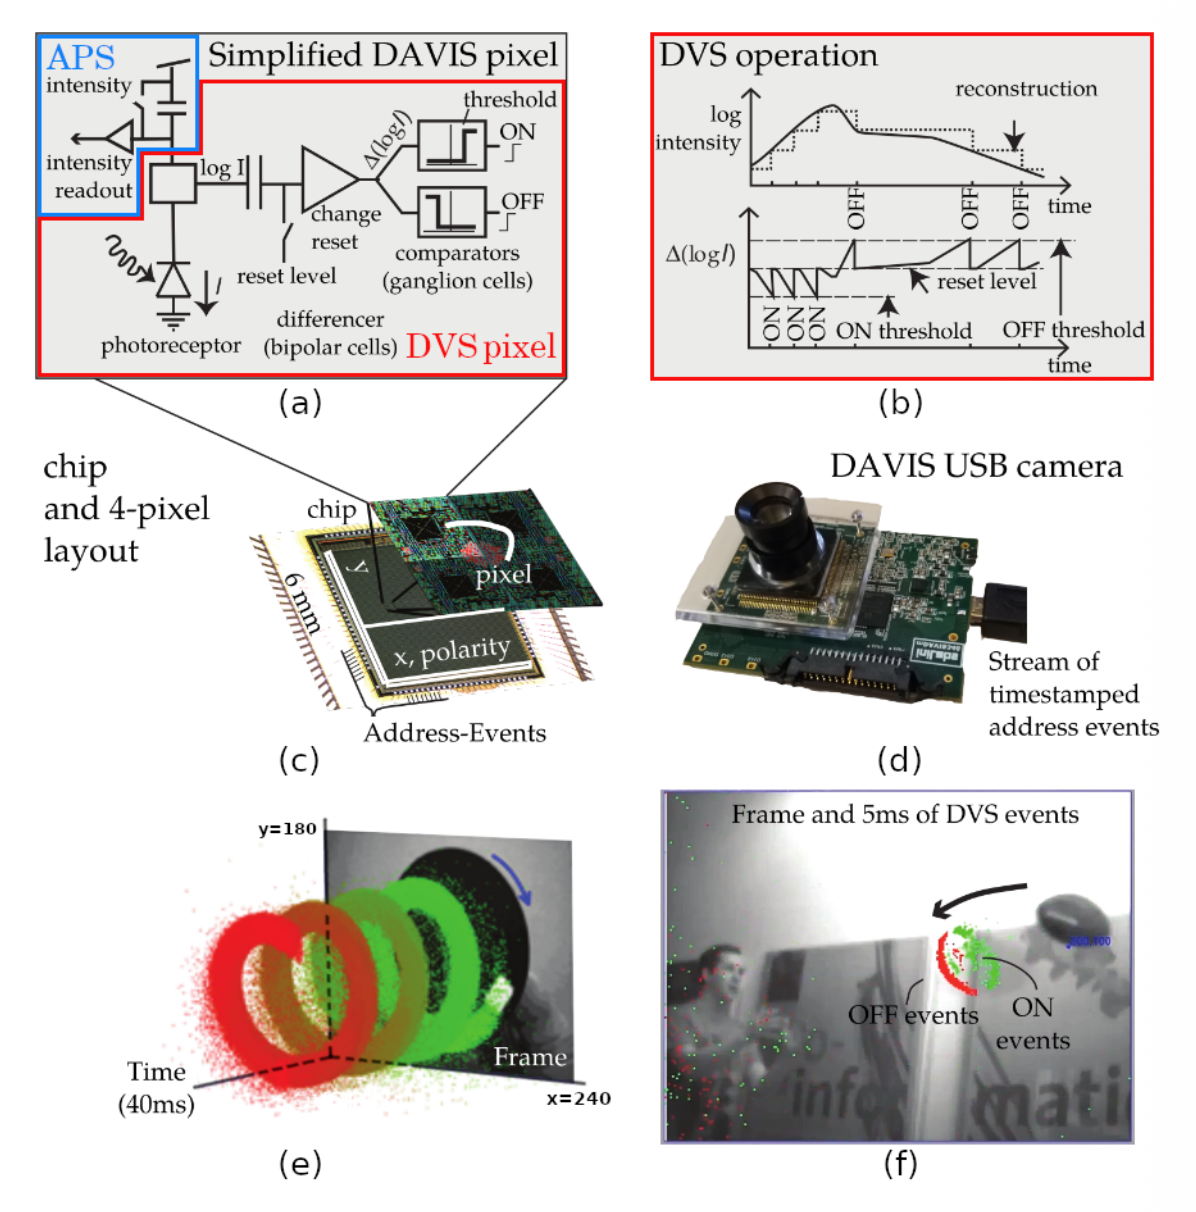
\includegraphics[width=0.75\textwidth]{images/fig_event_camera_principle.png}
    \caption{Operating principle of a Dynamic Vision Sensor (DVS). Each pixel independently and asynchronously fires an event when the change in log luminance exceeds a contrast threshold $C$, producing a stream of events $(x, y, t, p)$ with microsecond temporal resolution. Adapted from \cite{gallego2020event}.}
    \label{fig:dvs_principle}
\end{figure}




\section{Event Representations for Deep Learning}
A central challenge in applying deep learning to event camera data lies in bridging the gap between the asynchronous, sparse nature of event streams and the dense, regular tensor inputs expected by most neural network architectures. Several event representations have been developed to address this challenge, each embodying different trade-offs between information preservation and computational efficiency. 

The simplest representation is the event frame or event histogram, which accumulates events within a fixed time window into a two-dimensional grid where each pixel takes a value in {+1, 0, -1} based on event polarity \cite{gallego2020event}. While this representation is directly compatible with standard CNN architectures, it discards temporal information within the accumulation window, effectively reducing the event stream to a snapshot that loses the very temporal richness that distinguishes event cameras from conventional sensors. 

Voxel grids, proposed by Zhu et al. \cite{zhu2019unsupervised}, address this limitation by discretising the event stream into a three-dimensional spatio-temporal volume. Events are accumulated into B temporal bins, producing a tensor of dimensions B × H × W that preserves temporal ordering. This representation has been widely adopted in subsequent work, including the Events-to-Video (E2VID) reconstruction framework \cite{rebecq2019e2vid} and various optical flow estimation methods. The number of temporal bins B represents a tuneable parameter balancing temporal resolution against computational cost. 

\begin{figure}[ht]
    \centering
    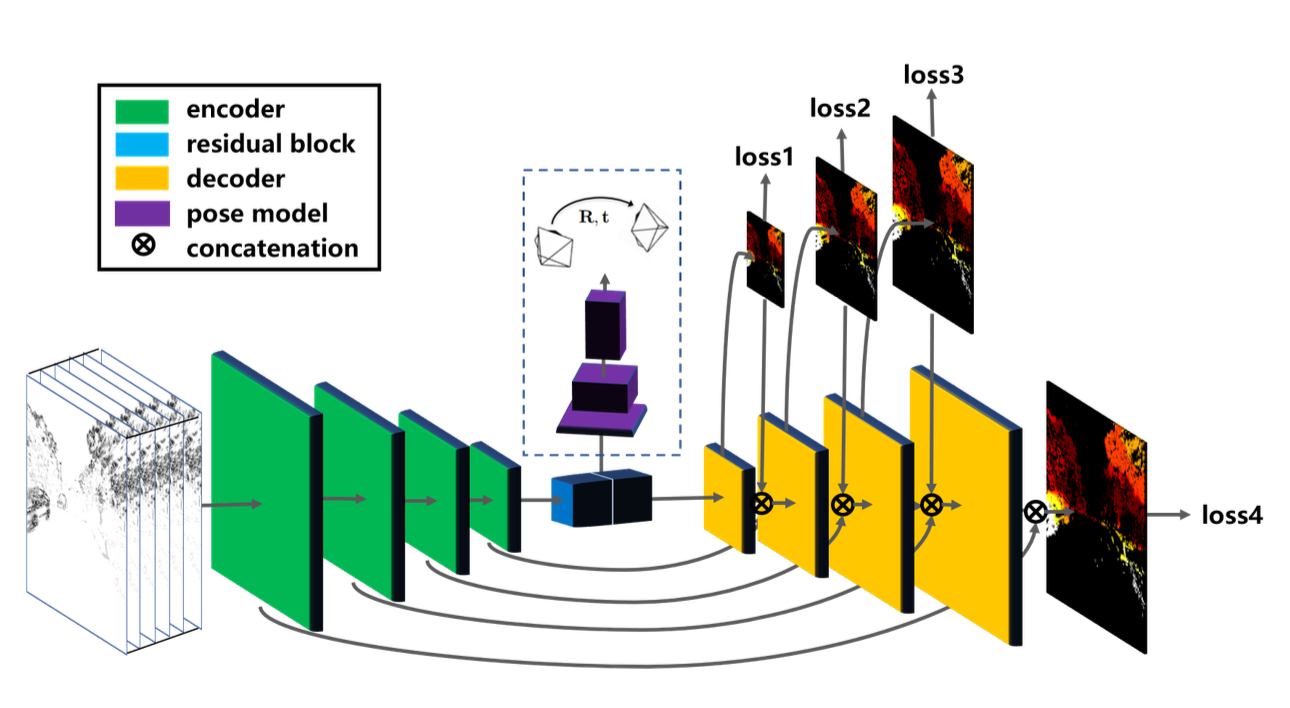
\includegraphics[width=0.75\textwidth]{images/fig_voxel_grid.png}
    \caption{Voxel grid event representation. Events within a fixed time window are accumulated into $B$ temporal bins, producing a tensor of shape $B \times H \times W$ that preserves temporal ordering. Each bin is normalised independently. Adapted from \cite{zhu2019unsupervised}.}
    \label{fig:voxel_grid}
\end{figure}

Time surfaces, introduced by Lagorce et al. \cite{lagorce2017hots}, offer an alternative encoding where each pixel stores an exponentially decaying function of the time since the last event at that location. This representation naturally encodes recency information and has been extended to Speed-Invariant Time Surfaces (SITS) that normalise for object velocity \cite{manderscheid2019speed}. Time surfaces are particularly effective for feature extraction and pattern recognition tasks, as they encode both spatial structure and temporal dynamics in a compact two-dimensional representation. 

Event Spike Tensors (ESTs), proposed by Gehrig et al. \cite{gehrig2019end}, sample the event stream using learned kernel functions, preserving temporal localisation with minimal information loss. Comparative studies have consistently demonstrated that representations retaining temporal localisation, such as voxel grids and ESTs, outperform simpler aggregation methods like event frames on downstream tasks \cite{gehrig2019end}. This finding underscores the importance of preserving the fine-grained temporal information inherent to event camera outputs. 

More recently, hybrid representations combining multiple channels of information have been explored. For instance, representations encoding polarity, timestamp, and event count in separate channels have shown improved performance on detection benchmarks \cite{innocenti2021temporal}. The choice of event representation remains an active area of research, with the optimal representation often being task-dependent. 

Among the representations surveyed, voxel grids are selected as the input representation for this work. Their three-dimensional spatio-temporal structure preserves temporal ordering across bins, a property demonstrated to be critical for detection performance \cite{gehrig2019end}, while remaining directly compatible with standard CNN and SSM-based backbone architectures. Time surfaces, although compact, collapse temporal structure into a single 2D map and are less suited to multi-object detection tasks where simultaneous events at different locations must be disambiguated. ESTs offer higher temporal fidelity through learned kernels, but introduce additional parameters and training complexity that is difficult to justify given the computational constraints of onboard UAV deployment. 

Hybrid multi-channel representations have shown promise on recent benchmarks \cite{innocenti2021temporal}, but require careful engineering of the channel structure and have not yet been validated on the Gen1 automotive dataset used in this work. A bin count of $B = 10$ is adopted throughout, consistent with prior work on the Gen1 dataset \cite{perot2020learning}, providing sufficient temporal resolution to capture object motion between detection frames without exceeding the memory budget of the target hardware platform. 

\section{Deep Learning for Event-Based Object Detection}
Object detection from event camera data has attracted growing research attention, with approaches broadly categorizable into four paradigms: frame-conversion methods that adapt standard detectors, spiking neural network (SNN) approaches, graph neural network (GNN) methods, and recurrent architectures that process events sequentially \cite{zheng2023deep}. 

\subsection{Frame-Conversion Approaches}
The most straightforward approach to event-based object detection converts event streams into frame-like representations and applies established detection architectures such as YOLO, SSD, or Faster R-CNN. Iacono et al. \cite{iacono2018towards} demonstrated that event histograms can be processed by standard object detectors with reasonable accuracy on automotive datasets. While this approach benefits from the maturity and optimisation of frame-based detection pipelines, it fundamentally fails to exploit the temporal continuity of the event stream, treating each accumulated frame independently. Furthermore, the frame accumulation step introduces latency that partially negates the low-latency advantage of event cameras. 

Perot et al. \cite{perot2020learning} introduced the Gen1 and 1Mpx automotive detection datasets and proposed a detection pipeline using learned event representations fed to an anchor-free detection head. Their work demonstrated that event cameras could achieve competitive detection performance in automotive scenarios, particularly under challenging lighting conditions where frame-based cameras struggle. However, the reliance on fixed-window accumulation remained a limiting factor.

\subsection{Spiking Neural Networks}
Spiking neural networks (SNNs) represent a bio-inspired approach that is architecturally well-matched to the asynchronous, binary nature of event camera outputs. In SNNs, information is encoded as discrete spikes rather than continuous activations, enabling highly energy-efficient computation on neuromorphic hardware \cite{roy2019towards}. The DT-LIF (Dual-Threshold Leaky Integrate-and-Fire) neuron model combined with the SSD detection framework, as proposed by Zhou et al. \cite{zhou2023dtlif}, demonstrated that SNNs can perform object detection from event data with significantly lower energy consumption than conventional neural networks. The dual-threshold mechanism improves the neuron's ability to encode temporal patterns by introducing separate thresholds for excitation and inhibition. 

More recently, the Hybrid Spiking Vision Transformer (HsVT) \cite{xu2025hybrid} has integrated spatial feature extraction with temporal spike-based processing, achieving competitive performance with fewer parameters and lower energy consumption than equivalent artificial neural networks. The key advantage of SNN-based detection for micro UAV applications lies in the potential for deployment on neuromorphic processors such as Intel's Loihi or SynSense's Speck chip, which offer orders-of-magnitude improvements in power efficiency compared to conventional GPUs \cite{synsense2026speck}. However, SNN training remains challenging due to the non-differentiability of spike generation, and detection accuracy generally lags behind state-of-the-art conventional architectures. 

\subsection{Graph Neural Networks}
An alternative paradigm models the event stream as a spatio-temporal graph, where individual events serve as nodes connected to their spatial and temporal neighbours. Graph neural networks (GNNs) can then extract features from this naturally sparse representation without requiring conversion to dense tensors \cite{bi2019graph}. The Asynchronous Event-based GNN (AEGNN) framework \cite{schaefer2022aegnn} demonstrated that graph-based processing preserves the asynchronous nature of events while enabling efficient feature extraction through graph convolutions and pooling operations. The primary advantage of GNN approaches is their ability to process events at their native resolution without temporal binning, potentially preserving more information than frame-based methods. However, the irregular memory access patterns of graph operations can be challenging to optimise on conventional hardware, and scalability to high event rates remains an open problem. 

\subsection{Recurrent Architectures}
Recurrent neural networks (RNNs), particularly those employing convolutional gated recurrent units (ConvGRUs), have been widely applied to sequential event processing. Recurrent architectures naturally accumulate temporal context across event windows, making them well-suited for tasks requiring temporal reasoning \cite{rebecq2019e2vid}, \cite{cannici2019attention}. The E2VID framework \cite{rebecq2019e2vid}, while primarily targeting video reconstruction, demonstrated that recurrent encoder-decoder networks with ConvGRU layers can effectively process temporal sequences of event representations. Several detection frameworks have adopted similar recurrent feature extractors to build temporal context for detection \cite{messikommer2020event}. 

The principal limitation of recurrent approaches for deployment on micro UAVs is their sequential processing requirement, which limits parallelisation and can create computational bottlenecks. Additionally, RNNs are known to struggle with very long temporal dependencies due to vanishing gradient problems, though gated variants partially mitigate this issue. Critically, Zubic et al. \cite{zubic2024state} demonstrated that RNN-based event processing models suffer significant performance degradation when deployed at inference frequencies different from their training frequency, a limitation that directly impacts the variable-rate nature of event camera data. 

\section{State Space Models: Architecture and Evolution}
State Space Models (SSMs) have recently emerged as a powerful class of sequence models that address many of the computational limitations of transformers and recurrent networks \cite{gu2022efficiently}. Rooted in control theory, SSMs model the relationship between an input sequence $u(t)$ and an output sequence $y(t)$ through a latent state $h(t)$ governed by a continuous-time linear dynamical system:

\begin{align}
    h'(t) &= Ah(t) + Bu(t) \\
    y(t) &= Ch(t) + Du(t)
\end{align}

where $A, B, C$, and $D$ are learnable parameter matrices \cite{gu2022efficiently}. This continuous-time formulation can be discretised at arbitrary time steps $\Delta t$ using methods such as the zero-order hold, enabling flexible adaptation to different sampling rates \cite{gu2022efficiently, zubic2024state}. 

The discretisation process transforms the continuous parameters $(A, B)$ into their discrete counterparts $(\overline{A}, \overline{B})$ using the step size $\Delta$:

\begin{equation}
    \overline{A} = \exp(\Delta A), \quad \overline{B} = (\exp(\Delta A) - I)A^{-1}B
\end{equation}

This allows the model to be computed as a linear recurrence, which is significantly more efficient for long sequences than the quadratic complexity of self-attention \cite{gu2023mamba, patro2025from}.

The Structured State Space Sequence Model (S4), proposed by Gu et al. \cite{gu2022efficiently}, represented a breakthrough by introducing a special parameterisation of the state matrix A based on the HiPPO (High-order Polynomial Projection Operator) framework. This parameterisation enables the efficient computation of very long-range dependencies while maintaining linear computational complexity in sequence length. S4 achieved state-of-the-art results on the Long Range Arena benchmark, including the challenging Path-X task with sequence lengths of 16,384, and attained 91\% accuracy on sequential CIFAR-10 \cite{gu2022efficiently}. The S5 variant \cite{smith2023simplified} further simplified the architecture by employing a diagonal state structure with parallel scan mechanisms, eliminating the need for computationally expensive FFT operations while maintaining comparable performance. 

\section{Mamba and Selective State Spaces}
The Mamba architecture, proposed by Gu and Dao \cite{gu2023mamba}, introduced a critical innovation: selective state spaces. Unlike the time-invariant S4 model, Mamba makes the matrices $B$, $C$, and the discretisation step $\Delta$ input-dependent, enabling the model to selectively attend to or ignore different parts of the input sequence based on content \cite{gu2023mamba}. This is achieved by defining these parameters as functions of the input $x_t$:

\begin{align}
    B_t &= \text{Linear}_B(x_t) \\
    C_t &= \text{Linear}_C(x_t) \\
    \Delta_t &= \text{Softplus}(\text{Parameter}_\Delta + \text{Linear}_\Delta(x_t))
\end{align}

This selectivity is analogous to the gating mechanisms in LSTMs and GRUs but operates within the SSM framework while maintaining linear computational complexity \cite{gu2023mamba}. Input-dependent $\Delta_t$ allows for selective retention: a large $\Delta_t$ causes the state to decay rapidly (resetting the memory for irrelevant content), while a small $\Delta_t$ preserves long-range memory \cite{gu2023mamba, zubic2024state}. 

To overcome the challenges of computing such a non-linear recurrence, Mamba employs a hardware-aware algorithm. This approach combines a parallel scan, kernel fusion, and selective recomputation to achieve 2--8$\times$ faster inference than comparable transformer models while matching their performance on competitive benchmarks \cite{gu2023mamba}. These efficiencies are particularly advantageous for the size, weight, and power (SWaP) constraints of micro-UAV platforms \cite{gu2023mamba, patro2025from}.

\begin{figure}[ht]
    \centering
    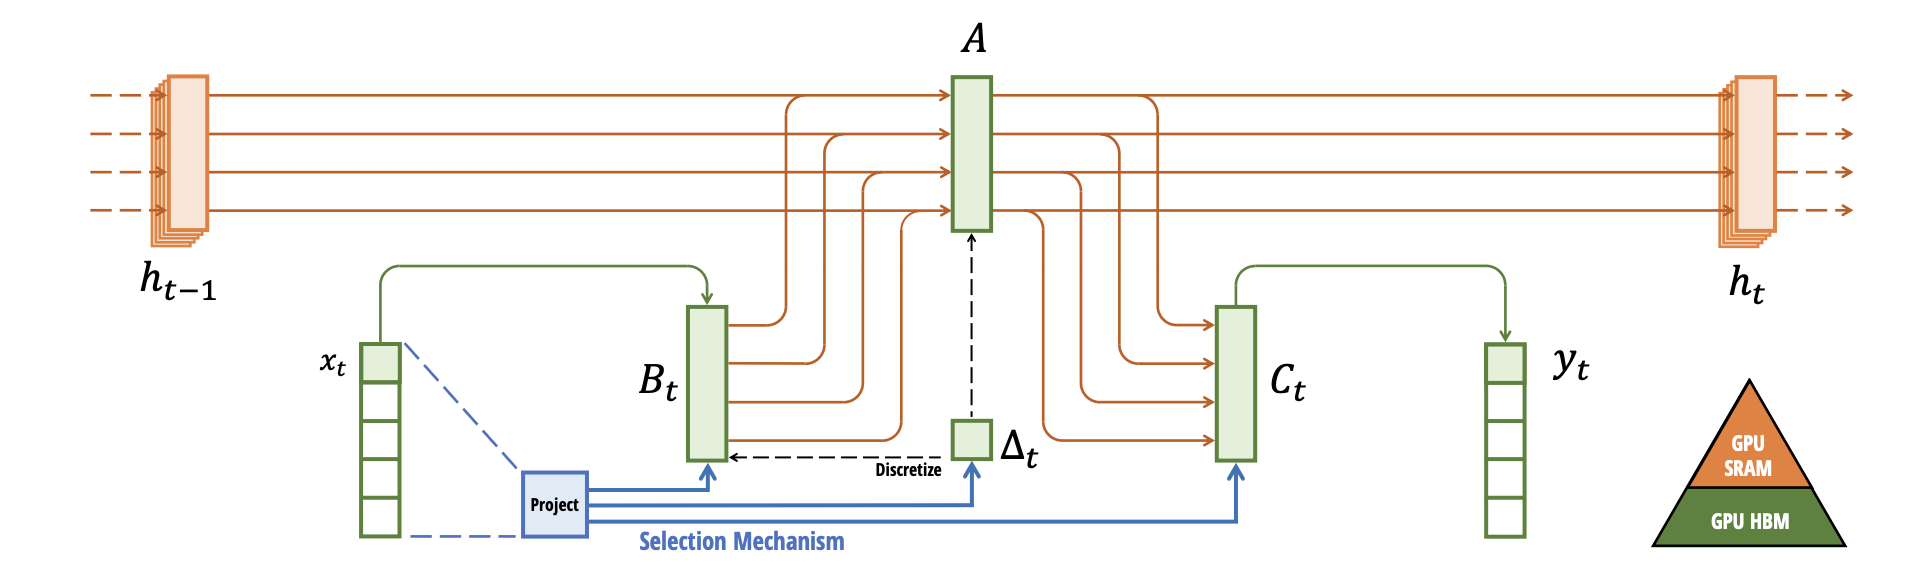
\includegraphics[width=0.85\textwidth]{images/fig_mamba_architecture.png}
    \caption{The Mamba selective state space model architecture. Input-dependent parameters $\Delta_t$, $B_t$, and $C_t$ are computed as functions of the input $x_t$, enabling content-aware selective retention of long-range temporal context while maintaining linear computational complexity. Adapted from \cite{gu2023mamba}.}
    \label{fig:mamba_arch}
\end{figure}

The extension of SSMs to vision tasks has proceeded rapidly. Vision Mamba (Vim) \cite{zhu2024vision} proposed a vision backbone employing bidirectional Mamba blocks with position embeddings, achieving 2.8× faster inference than the DeiT transformer on ImageNet while using 86.8\% less GPU memory for high-resolution image processing. VMamba \cite{liu2024vmamba} introduced Visual State-Space (VSS) blocks with a 2D Selective Scan (SS2D) module that traverses image patches along multiple scan paths to capture two-dimensional spatial relationships. PlainMamba \cite{yang2024plainmamba} further explored non-hierarchical Mamba structures for visual recognition. These vision SSMs consistently demonstrate that the linear complexity of state space models can be leveraged for visual tasks without sacrificing the representational capacity needed for accurate perception. 

The computational advantages of SSMs are particularly relevant for micro UAV applications. The O(n) complexity of SSMs, compared to the O(n²) complexity of transformers, directly translates to reduced inference time and memory consumption. Furthermore, the continuous-time formulation of SSMs allows deployment at variable time scales without retraining, a property that Zubic et al. \cite{zubic2024state} have shown to be uniquely advantageous for event camera data where the effective data rate varies with scene dynamics. A comprehensive survey by Patro et al. \cite{patro2025from} has catalogued the rapid evolution from S4 to Mamba and its variants, documenting the expanding application of SSMs across vision, language, and multi-modal tasks. 

\section{State Space Models for Event Camera Data}
The intersection of SSMs and event-based vision is a nascent but rapidly developing area. Zubic et al. \cite{zubic2024state} presented the first systematic investigation of SSMs for event camera data, published as a CVPR 2024 Spotlight paper. Their work identified a fundamental limitation of existing deep learning approaches to event data: when trained at one temporal resolution (i.e., a specific ratio between the number of events and the number of forward passes of the network), models based on CNNs, RNNs, and transformers all exhibit significant performance degradation when deployed at different temporal resolutions. This is particularly problematic for event cameras, where the event rate naturally varies with scene dynamics. 

Zubic et al. \cite{zubic2024state} demonstrated that SSMs, viewed as linear time-invariant (LTI) continuous-time systems, can be discretised at arbitrary step sizes without retraining. By introducing a learnable global timescale parameter that adjusts based on the ratio between training and inference frequencies, their SSM-based models maintained performance across a range of deployment frequencies with minimal degradation (3.76 mAP drop versus >20 mAP for RNNs and transformers at higher frequencies). Furthermore, the SSM approach achieved 33\% faster training compared to equivalent recurrent models. These results provide strong evidence that SSMs are architecturally well-suited to the temporal characteristics of event camera data. 

The most influential baseline for event-based object detection is the Recurrent Vision Transformer (RVT) introduced by Gehrig and Scaramuzza \cite{gehrig2023recurrent}. RVT employs a four-stage hierarchical backbone combining convolutional priors with local and dilated global self-attention, using a ConvLSTM to carry hidden state across consecutive 50~ms windows \cite{gehrig2023recurrent}. A Feature Pyramid Network (FPN) and YOLOX detection head complete the pipeline \cite{gehrig2023recurrent}. 

RVT achieved $47.2$~mAP on the Gen1 automotive dataset with an inference latency below 12~ms, a five-fold reduction compared to prior art \cite{gehrig2023recurrent}. All subsequent SSM-based methods, including those explored in this work, benchmark against RVT, making it the de facto reference architecture for this thesis \cite{gehrig2023recurrent, zubic2024state, yang2025smamba}.

Zubic et al. \cite{zubic2024state}, described above, apply SSMs directly within the RVT framework for event-based object detection, achieving 47.71 mAP on Gen1 with S5 layers replacing the ConvLSTM. Critically, the SSM is used purely for inter-frame temporal aggregation; spatial feature extraction remains handled by Transformer attention blocks. The SSM variant employed is S5, a fixed-parameter (non-selective) model whose transition matrices do not depend on the input. 

Most recently, SMamba \cite{yang2025smamba} (AAAI 2025) advances the state of the art on Gen1 to 50.4 mAP by replacing the spatial Transformer stages of RVT with a Sparse Selective Mamba (S6) backbone. A Spatio-Temporal Continuity Assessment (STCA) module identifies informative tokens and discards noisy or inactive patches before the Mamba scan, reducing FLOPs by 23\% while improving accuracy. Inter-frame temporal context is still provided by a ConvLSTM, not Mamba. SMamba thus demonstrates that selective Mamba outperforms fixed-parameter SSMs for spatial feature extraction in event-based detection. 

Despite this progress, a consistent pattern emerges across all top-performing methods: every SOTA architecture maintains inter-frame recurrence (LSTM or SSM hidden state across consecutive windows) and uses multi-scale FPN detection. No prior work has evaluated a fully recurrence-free selective Mamba architecture for event-based detection, nor conducted a controlled ablation comparing a CNN-SSM hybrid against a pure SSM model under identical experimental conditions. These constitute the primary architectural contributions of this thesis. The application of SSM-based event detection to micro-UAV platforms with SWaP constraints additionally has no prior demonstration.

\section{Event-Based Vision for UAV Navigation and Obstacle Avoidance}
The application of event cameras to UAV navigation has been an active area of research, driven by the sensor's inherent advantages for high-speed, low-latency perception. Pioneering work in event-based visual odometry (EVO) by Rebecq et al. \cite{rebecq2017real} demonstrated that event cameras could provide accurate ego-motion estimation, a fundamental capability for UAV localisation. Their approach tracked features generated by events to estimate the 6-DOF pose of the camera, achieving robust performance in scenarios with rapid motion and high dynamic range that caused frame-based visual odometry methods to fail. 

Vidal et al. \cite{vidal2018ultimate} extended this work by combining event-based visual odometry with depth estimation, demonstrating that event cameras could provide the 3D environmental understanding necessary for obstacle-aware navigation. Their monocular depth estimation approach used transfer learning from conventional vision datasets to event-based depth prediction, achieving high-quality depth maps suitable for navigation planning. 

Falanga et al. \cite{falanga2019fast} presented a seminal contribution in event-based obstacle avoidance for quadrotors. Their approach performed motion segmentation on the event stream to identify independently moving objects, then computed time-to-contact estimates to trigger avoidance manoeuvres. The system achieved an overall processing latency of approximately 3.5 milliseconds, enabling the quadrotor to avoid obstacles at relative speeds up to 10 m/s. Critically, their work demonstrated that event cameras could enable reactive obstacle avoidance at speeds far beyond the capabilities of frame-based perception systems, where the minimum achievable latency is bounded by the frame rate (typically 30-60 ms per frame). 

Sanket et al. \cite{sanket2020evdodgenet} proposed EVDodge, an event-based dodging system tested on UAV platforms. Their approach demonstrated real-time obstacle avoidance using purely event-based perception, showing that the high temporal resolution of event cameras could be directly translated into improved avoidance performance. The system was validated both in simulation and on physical quadrotor platforms, confirming the practical feasibility of event-based avoidance systems. 

More recent work has explored bio-inspired processing pipelines for event-based UAV obstacle avoidance. Li et al. \cite{li2024taming} proposed a neuromorphic processing architecture that integrates event camera data with bio-inspired algorithms running on dedicated neuromorphic hardware, achieving real-time obstacle avoidance with power consumption in the milliwatt range. This approach is particularly relevant for micro UAVs where power budget is a primary constraint. 

Despite these advances, each of the surveyed approaches has notable limitations. The visual odometry and motion segmentation methods of Rebecq et al.\ \cite{rebecq2017real} and Falanga et al.\ \cite{falanga2019fast} use handcrafted features and geometric rules rather than learned representations, which limits how well they generalise to new environments. EVDodge \cite{sanket2020evdodgenet}, while shown to work on real hardware, uses a relatively shallow network that has not been tested under challenging conditions such as cluttered scenes or rapidly changing lighting. The neuromorphic approach of Li et al.\ \cite{li2024taming} is attractive for its low power consumption, but depends on specialised hardware that is not yet available at the micro-UAV scale and cannot easily support the kind of spatial feature extraction required for general object detection. Most importantly, none of these methods combine learned deep spatial features with a temporal model that can handle variable event rates, the core gap that this thesis addresses through its SSM-based detection architecture. 

\section{Contrast Maximisation and Motion Estimation from Events}
Gallego et al. \cite{gallego2018unifying} proposed a unifying contrast maximisation framework for event-based vision that provides a principled approach to estimating motion, depth, and optical flow from events. The core idea is to warp events according to a candidate motion model and measure the contrast (sharpness) of the resulting warped event image; the motion parameters that maximise contrast correspond to the true motion. This framework elegantly handles the data association problem inherent in event-based motion estimation without requiring explicit feature matching or appearance information. 

The contrast maximisation principle has been extended and refined by subsequent work. Shiba et al. \cite{shiba2024secrets} applied it to dense optical flow, depth, and ego-motion estimation, introducing multi-scale approaches to improve convergence and better handle occlusions. Self-supervised learning-based optical flow methods, such as EV-FlowNet \cite{zhu2018evflownet}, have also been developed, using photometric losses as supervisory signals to learn event-to-flow mappings without requiring ground truth annotations. These motion estimation capabilities are directly relevant to obstacle avoidance, as optical flow and time-to-contact can be used to identify and respond to approaching obstacles.

\section{Event Camera Datasets and Benchmarks}
The availability of standardised datasets has been instrumental in advancing event-based vision research. Several benchmark datasets are relevant to the object detection and navigation tasks considered in this thesis. 

The DSEC dataset \cite{gehrig2021dsec}, developed at the University of Zurich, provides high-resolution stereo event camera data captured using Prophesee Gen3.1 sensors with a 60 cm baseline, complemented by global shutter colour cameras and LiDAR ground truth. DSEC covers a range of driving scenarios under both favourable and challenging illumination conditions, making it a valuable benchmark for event-based depth estimation and optical flow. 

The MVSEC (Multi Vehicle Stereo Event Camera) dataset \cite{zhu2018multivehicle} uses DAVIS346B stereo pairs with a 10 cm baseline, providing synchronised event, frame, IMU, and LiDAR data. MVSEC includes sequences from indoor flying, outdoor driving, and motorcycle scenarios, offering diverse conditions for evaluating perception algorithms. 

For object detection specifically, the Gen1 and 1Mpx datasets \cite{perot2020learning} provide large-scale event camera recordings with bounding box annotations for cars and pedestrians, captured using Prophesee event cameras in automotive settings. The N-Caltech101 dataset \cite{orchard2015converting} provides an event camera version of the Caltech101 classification benchmark, created by displaying images on a monitor in front of a DVS camera executing saccadic movements. While primarily a classification benchmark, N-Caltech101 has been widely used for evaluating event representation and feature extraction methods. 

A significant gap exists in available datasets for UAV-specific scenarios. Most event camera datasets target automotive applications, and there are limited publicly available datasets that capture the specific challenges of micro UAV navigation: rapid ego-motion, indoor environments, small obstacles, and the particular motion patterns characteristic of rotary-wing flight. Addressing this dataset gap remains an open challenge for UAV-specific event-based perception research. For the purposes of this thesis, the primary evaluation is conducted on the Gen1 automotive dataset, which provides a well-established benchmark for detection performance. Obstacle avoidance is treated as a motivating application rather than a directly evaluated system the trained detection model represents the core perceptual component that such a system would require. Extension to UAV-specific scenarios, potentially through synthetic data generation in open-source simulators such as Gazebo with event camera emulation, is identified as a direction for future work subject to hardware and time constraints. 

\section{Computational Constraints and Obstacle Avoidance for Micro UAVs}
Micro UAVs in the sub-250 gram class face severe SWaP constraints that fundamentally shape the design of onboard perception systems. Typical computational platforms for micro UAVs include ARM Cortex-M class microcontrollers with as little as 192 kB of memory \cite{niculescu2022improving}, which are orders of magnitude less capable than the GPU-equipped systems used to train and evaluate most deep learning models. This disparity between training and deployment hardware necessitates either highly efficient model architectures, hardware acceleration, or offloading computation to a ground station at the cost of communication latency. 

Several approaches to obstacle avoidance on resource-constrained platforms have been explored. Traditional methods based on optical flow divergence or time-to-contact estimation provide computationally lightweight avoidance capabilities but lack the ability to classify or localise specific obstacles \cite{falanga2019fast}, \cite{decroon2016monocular}. Model predictive control (MPC) approaches can generate optimal avoidance trajectories but require real-time environmental perception as input. Cooperative approaches, where a less-equipped micro UAV receives guidance from a sensor-rich companion \cite{petracek2024drones}, offer a pragmatic solution but introduce communication dependencies. 

The emergence of neuromorphic processing hardware offers a potential path to efficient onboard perception. The SynSense Speck chip \cite{synsense2026speck} integrates a dynamic vision sensor with a fully asynchronous spiking neural network processor, achieving real-time event processing with idle power consumption below 1 mW. Similarly, Intel's Loihi 2 neuromorphic processor supports on-chip learning and efficient SNN inference \cite{davies2021advancing}. These platforms are particularly well-suited to processing event camera data, as they natively handle the sparse, asynchronous data format. However, the software ecosystem for neuromorphic processors remains immature compared to conventional deep learning frameworks, and mapping complex detection architectures onto neuromorphic hardware remains an active research challenge. 

The linear complexity and inherent efficiency of SSM-based architectures position them as strong candidates for deployment on the limited computational resources available on micro UAVs. Unlike transformer-based models that require quadratic memory and computation, SSMs can process long event sequences with predictable and modest resource requirements. Combined with model compression techniques such as quantisation and pruning, SSM architectures may enable real-time object detection on platforms that cannot support transformer or large CNN inference. 

\section{Identification of Research Gaps}
The preceding review reveals several interconnected research gaps that this thesis aims to address: 

Gap 1: Pure selective Mamba for event-based object detection. Existing SSM-based detection methods integrate SSM layers into Transformer backbones \cite{zubic2024state} or employ selective Mamba within sparse-attention hybrid frameworks \cite{yang2025smamba}. In both cases, inter-frame recurrence is maintained via ConvLSTM or SSM hidden state passed across consecutive windows. No prior work has evaluated a fully recurrence-free, convolutional-free selective Mamba architecture for event-based detection, nor conducted a controlled ablation comparing a CNN-SSM hybrid against a pure SSM model under identical loss functions, detection heads, and training protocols. Such a comparison is required to isolate the contribution of the spatial feature extractor from all other architectural variables. 

Gap 2: Integrated detection and avoidance for micro UAVs. Existing event-based UAV obstacle avoidance systems \cite{falanga2019fast, sanket2020evdodgenet} predominantly employ reactive strategies based on optical flow or motion segmentation, without explicit object detection. Conversely, event-based detection methods \cite{perot2020learning,gehrig2023recurrent} have been evaluated primarily on automotive benchmarks. An integrated system that combines SSM-based object detection with obstacle avoidance control, specifically designed for micro UAV deployment, has not been demonstrated. 

Gap 3: Computational efficiency benchmarking for onboard deployment. While the theoretical computational advantages of SSMs over transformers and RNNs are well-established, systematic benchmarking of SSM inference latency, memory consumption, and energy usage on the constrained hardware platforms typical of micro UAVs has not been conducted. Understanding the practical deployment characteristics of SSM-based detection models is essential for validating their suitability for this application domain. 

Gap 4: Variable-rate event processing for obstacle avoidance. The unique ability of SSMs to generalise across temporal resolutions \cite{zubic2024state} has not been exploited in the context of obstacle avoidance, where the event rate varies dramatically with UAV speed and scene complexity. An adaptive processing framework that adjusts its temporal resolution based on event rate while maintaining detection performance could significantly improve both efficiency and robustness. 

These gaps collectively define the research space for this thesis: developing and evaluating SSM-based architectures for event-based object detection and obstacle avoidance on micro UAVs, with a focus on computational efficiency, temporal adaptability, and practical deployability. 


% --- Chapter 3: Methodology ---
\chapter{Research Question and Project Plan} 

\section{Research Question}
The central research question of this thesis is: Can State Space Model architectures effectively process event camera data for real-time object detection and autonomous obstacle avoidance on resource-constrained micro UAVs, and do they offer measurable advantages over existing CNN, RNN, and transformer-based approaches in terms of detection accuracy, computational efficiency, and temporal adaptability? 

\section{Hypothesis and Aims}
Primary Hypothesis: SSM-based architectures, by virtue of their linear computational complexity and natural compatibility with variable-rate temporal data, will achieve detection accuracy comparable to or exceeding state-of-the-art recurrent and transformer-based methods on event camera object detection benchmarks, while requiring significantly fewer computational resources suitable for micro-UAV deployment \cite{gu2023mamba, zubic2024state}.

The research objectives are decomposed into the following specific aims:

\begin{description}
    \item[\textbf{Aim 1: Architecture Development}] \hfill \\
    Develop an SSM-based object detection architecture for event camera data, evaluating candidate SSM variants ($S4, S5$, Mamba) as temporal feature extractors within a detection framework \cite{gu2022efficiently, smith2023simplified, gu2023mamba}.
    
    \item[\textbf{Aim 2: Comparative Benchmarking}] \hfill \\
    Benchmark the proposed architecture against CNN, RNN, and transformer baselines on established event camera detection datasets (Gen1, 1Mpx) \cite{perot2020learning}. Metrics will include detection accuracy (mAP), inference latency, memory consumption, and energy usage.
    
    \item[\textbf{Aim 3: Temporal Generalisation}] \hfill \\
    Evaluate the temporal generalisation capability of the SSM-based detector by testing performance across different event accumulation frequencies without retraining, leveraging the continuous-time properties of SSMs \cite{zubic2024state}.
    
    \item[\textbf{Aim 4: System Integration}] \hfill \\
    Integrate the SSM-based detection module with an obstacle avoidance control framework and evaluate the end-to-end system in simulation (e.g., Gazebo/AirSim) and, if feasible, on a physical micro-UAV platform \cite{falanga2019fast, sanket2020evdodgenet}.
\end{description}

\section{Proposed Methodology}
The proposed methodology consists of four phases, detailed below. 

\subsection{Phase 1: Architecture Design and Implementation}
The first phase involves designing an SSM-based detection architecture for event camera data. The architecture will use a backbone consisting of SSM blocks (evaluating S4, S5, and Mamba variants) that process temporal sequences of event representations (voxel grids or ESTs) to extract spatio-temporal features. These features will be fed to a detection head (anchor-free, following the approach of Perot et al. \cite{perot2020learning}) to produce object bounding boxes and class predictions. The architecture will be implemented in PyTorch, leveraging existing SSM implementations from the mamba-ssm and state-spaces libraries. 

\subsection{Phase 2: Training and Benchmarking}
The detection model will be trained on the Gen1 and 1Mpx event camera object detection datasets \cite{perot2020learning}, which provide bounding box annotations for cars and pedestrians. Training will use standard protocols with data augmentation techniques adapted for event data. Performance will be benchmarked against published baselines including: a CNN-based detector with event frames, a ConvGRU-based recurrent detector, and a transformer-based detector. Metrics will include mean average precision (mAP), inference latency on both GPU and embedded hardware (e.g., NVIDIA Jetson Nano as a proxy for micro UAV compute), and model parameter count. 

\subsection{Phase 3: Temporal Generalisation Evaluation}
Following the protocol of Zubic et al. \cite{zubic2024state}, the trained model will be evaluated at inference frequencies ranging from 0.5× to 4× the training frequency, measuring mAP degradation as a function of frequency ratio. This experiment will quantify the practical advantage of SSMs for variable-rate event processing compared to RNN and transformer baselines. 

\subsection{Phase 4: Obstacle Avoidance Integration}
The SSM-based detector will be integrated with a reactive obstacle avoidance controller within a simulated micro UAV environment using AirSim or Gazebo with event camera simulation plugins. The avoidance system will use detection outputs (bounding boxes and estimated distances) to compute avoidance trajectories. Performance will be evaluated in terms of collision rate, avoidance latency, and trajectory smoothness across scenarios of varying complexity. If time and resources permit, preliminary hardware testing on a physical micro UAV platform equipped with an event camera will be conducted.  

\section{Thesis Timeline}
The project spans three thesis terms divided into eight phases, from literature review through to final submission. The full phase breakdown and week-by-week Gantt chart are provided together in Appendix~\ref{app:gantt}.

\section{Available Resources}
The following resources have been identified as essential and available for the successful completion of this project:
\begin{enumerate}
    \item \textbf{Computational Hardware:} UNSW's high-performance computing cluster (Katana) with GPU nodes for large-scale model training, supplemented by a personal workstation with an AMD Radeon RX 7700 XT GPU (ROCm backend) for local development.
    \item \textbf{Event Camera Hardware:} DAVIS346 and Prophesee Gen3.1 event cameras are available through the UNSW School of Mechanical and Manufacturing Engineering laboratory. Access requires completion of standard lab inductions. The DAVIS346 is selected as the primary platform; the Prophesee sensors are not used due to cost constraints that preclude their deployment on a physical micro UAV.
    \item \textbf{Datasets:} Standardised event camera datasets including Gen1, 1Mpx, DSEC, MVSEC, and N-Caltech101.
    \item \textbf{Software Ecosystem:} Open-source libraries including PyTorch, \texttt{mamba-ssm}, S4/S5 implementations, and event camera plugins for AirSim/Gazebo.
    \item \textbf{UAV Platforms:} Micro-UAV hardware available through the School of Mechanical and Manufacturing Engineering’s robotics laboratory.
\end{enumerate}

\section{Required Training and Upskilling}
To address the technical complexity of this work, the following upskilling areas have been identified:
\begin{enumerate}
    \item \textbf{SSM Implementation:} Developing expertise in the implementation and training of Mamba and other state space architectures.
    \item \textbf{Simulation Environments:} Configuring and utilizing AirSim or Gazebo for high-fidelity UAV and event sensor simulation.
    \item \textbf{Embedded Optimisation:} Learning model compression techniques, including quantisation and pruning, for resource-constrained deployment.
    \item \textbf{Safety and Risk Management:} Obtaining necessary certifications for safe micro-UAV operation and following strict flight protocols.
\end{enumerate}

% --- Chapter 4: Preliminary Preparations ---
\chapter{Project Dependent Preparations} 

\section{Literature and Software Familiarisation}
Substantial progress has been made across the literature review, software preparation, and MVP implementation phases. The literature review has been completed, with over 50 papers surveyed and catalogued across the domains of event-based vision, state space models, object detection, and UAV obstacle avoidance. The software development environment has been configured and verified on Apple Silicon (M4) hardware using PyTorch 2.3 with the Metal Performance Shaders (MPS) backend, confirming cross-platform compatibility for local development prior to full-scale training on the UNSW Katana HPC cluster. An end-to-end MVP codebase has been implemented, encompassing event data preprocessing (voxel grid representation), the S5-RVT baseline architecture, an anchor-free multi-class detection and classification head, training infrastructure with AdamW optimisation and gradient clipping, and mean Average Precision (mAP) evaluation. The codebase is modular and structured for extension to the two novel architectures and full training on the Gen1 automotive event camera dataset in Thesis~B. 

\section{MVP: Baseline Reproduction - Zubic et al.\ (2024)}
\label{sec:mvp}

\subsection{Motivation and Strategy}
\label{subsec:mvp_motivation}

The MVP phase of this thesis adopts a reproduction-first strategy. Rather than training a novel architecture from scratch, the MVP reproduces the published S5-RVT pipeline of Zubic et al.\ \cite{zubic2024state}, a CVPR 2024 Spotlight paper that represents the current state of the art in SSM-based event-camera object detection. This approach achieves two objectives: it produces a concrete, verifiable performance baseline on the Gen1 benchmark dataset, and it provides an end-to-end evaluation pipeline that can be directly extended to support the custom architecture ablation study in Thesis~B.

The decision to reproduce rather than train from scratch is methodologically justified. Training large event-based detection models from random initialisation requires substantial GPU time and dataset preparation; these resources are better deployed in Thesis~B once the research direction is confirmed. Reproducing a published result first ensures that the evaluation pipeline is correct, the dataset preprocessing is consistent with the literature, and the mAP numbers are directly comparable to those reported in peer-reviewed sources.

\subsection{Architecture: S5-RVT}
\label{subsec:mvp_arch}

Zubic et al.\ \cite{zubic2024state} modify the Recurrent Vision Transformer (RVT) baseline \cite{gehrig2023recurrent} by replacing its ConvLSTM inter-frame recurrence with an S5 (Simplified Structured State Space) layer. The resulting S5-RVT architecture processes sequences of event voxel grids through four stages:

\begin{enumerate}
    \item \textbf{Event Representation:} Raw events are accumulated into 10-bin voxel grids of shape $10 \times H \times W$ over fixed 50~ms windows.
    \item \textbf{Spatial Feature Extraction:} A four-stage hierarchical backbone combining convolutional priors with local and dilated global self-attention extracts multi-scale spatial features.
    \item \textbf{Temporal Aggregation:} Hidden state is propagated across consecutive windows using S5 layers rather than ConvLSTM, enabling the model to exploit the continuous-time discretisation properties of SSMs.
    \item \textbf{Detection Head:} A Feature Pyramid Network (FPN) and YOLOX-style anchor-free detection head produce bounding box predictions for cars and pedestrians.
\end{enumerate}

\begin{figure}[ht]
    \centering
    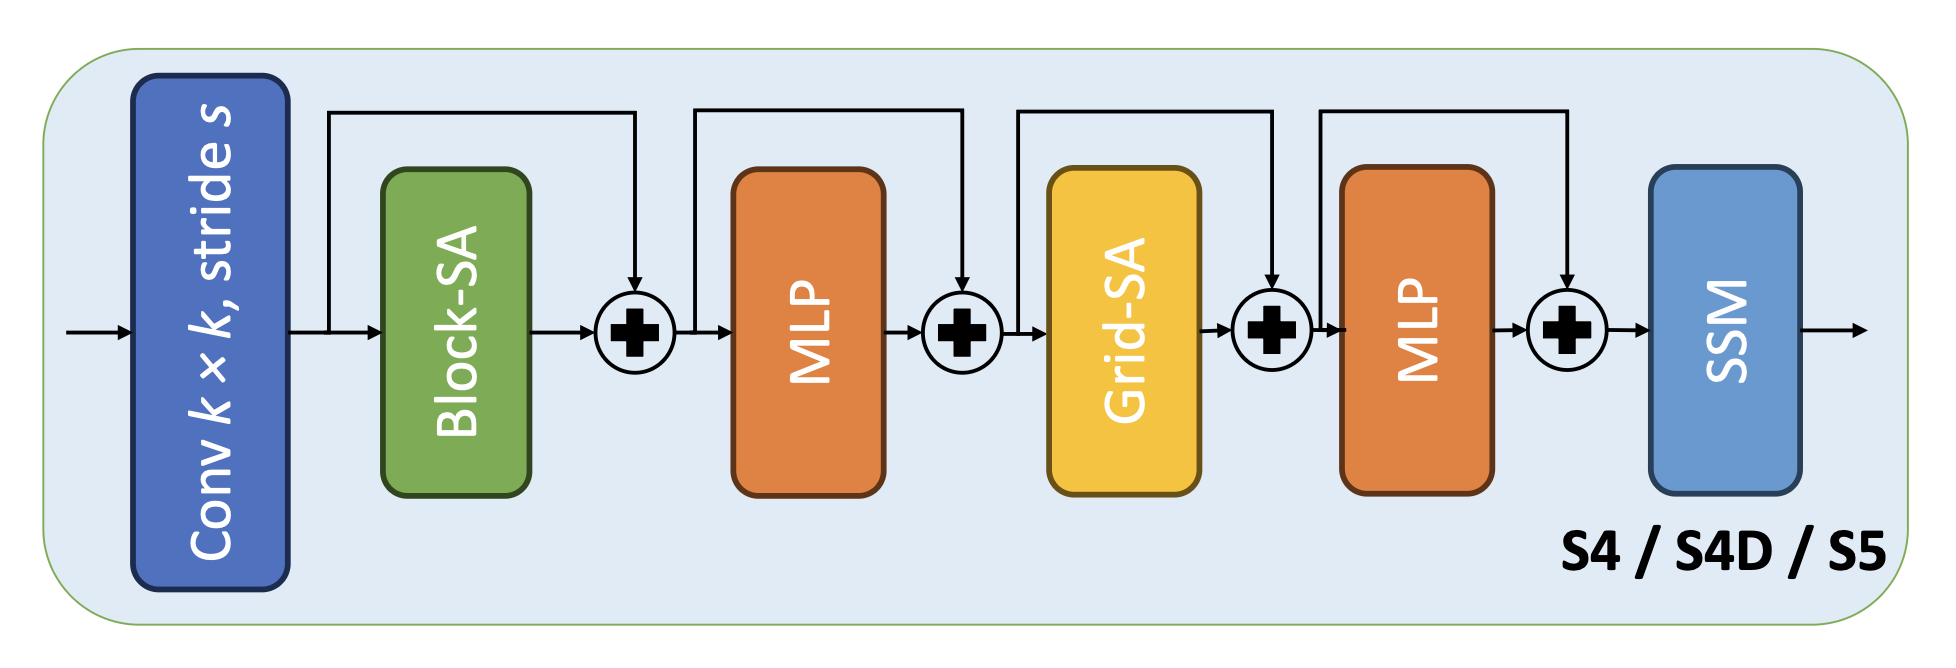
\includegraphics[width=0.85\textwidth]{images/fig_s5rvt_architecture.png}
    \caption{S5-RVT architecture. The Recurrent Vision Transformer backbone processes sequences of event voxel grids through four hierarchical stages. The ConvLSTM inter-frame recurrence of the original RVT \cite{gehrig2023recurrent} is replaced by an S5 State Space Model layer, enabling temporal generalisation across variable event rates. Reproduced from \cite{zubic2024state}.}
    \label{fig:s5rvt}
\end{figure}

The key theoretical advantage of S5 over ConvLSTM is its arbitrary discretisation step size: by adjusting the timescale parameter $\Delta$, the model can be deployed at inference frequencies different from the training frequency without retraining \cite{zubic2024state}. This property is uniquely relevant to event cameras, where the effective event rate varies with scene dynamics and UAV speed.

\subsection{Experimental Setup}
\label{subsec:mvp_setup}

\textbf{Dataset.} Evaluation is performed on the Prophesee Gen1 automotive detection dataset \cite{perot2020learning}, comprising event streams from a 240$\times$304 pixel event camera with bounding box annotations for cars and pedestrians. The official test split is used for all reported results, consistent with the evaluation protocol of Zubic et al.\ \cite{zubic2024state}.

\textbf{Model Variant.} The S5-ViT-Base checkpoint, trained for 100 epochs on Gen1 by the original authors, is used without further fine-tuning. This directly replicates the setting reported in Table~1 of \cite{zubic2024state}.

\textbf{Hardware.} Evaluation was performed on an AMD Radeon RX~7700~XT GPU (12~GB VRAM) running ROCm~6.4.2 under Ubuntu~22.04, using PyTorch~2.2.1 with the ROCm backend.

\textbf{Evaluation Metric.} Mean Average Precision at IoU threshold 0.5 (mAP@0.5), computed over the two target classes, following the standard protocol for this benchmark.

\subsection{Results}
\label{subsec:mvp_results}

Table~\ref{tab:mvp_results} reports the per-class and overall mAP@0.5 obtained from the evaluation run.

\begin{table}[H]
\centering
\caption{S5-RVT (ViT-Base) evaluation results on the Gen1 test set. Results reproduce Zubic et al.\ \cite{zubic2024state}.}
\label{tab:mvp_results}
\renewcommand{\arraystretch}{1.4}
\begin{tabular}{lcc}
\toprule
\textbf{Class} & \textbf{AP@0.5} & \textbf{Reference} \\
\midrule
Car         & 56.8  & 56.8 \\
Pedestrian  & 38.6  & 38.6 \\
\midrule
\textbf{Overall mAP@0.5} & \textbf{47.7} & \textbf{47.71} \\
\bottomrule
\end{tabular}
\end{table}

The reproduced result is within 0.01 mAP@0.5 of the published figure, confirming that the evaluation pipeline is correctly configured and that the dataset preprocessing is consistent with the original paper. Minor deviations from the published result may arise from hardware-specific numerical precision differences between ROCm and CUDA execution environments. These results establish S5-RVT as the performance baseline for all subsequent comparisons in Thesis~B.

Table~\ref{tab:state_of_art_compare} contextualises the MVP result against the broader state of the art.

\begin{table}[h]
\centering
\caption{State-of-the-art comparison on Gen1 mAP@0.5. MVP result in bold.}
\label{tab:state_of_art_compare}
\renewcommand{\arraystretch}{1.4}
\begin{tabular}{llcc}
\toprule
\textbf{Model} & \textbf{Recurrence} & \textbf{mAP@0.5} & \textbf{Venue} \\
\midrule
RVT \cite{gehrig2023recurrent}          & ConvLSTM  & 47.2  & CVPR 2023 \\
\textbf{S5-RVT \cite{zubic2024state}}   & \textbf{S5 SSM}    & \textbf{47.7} & \textbf{CVPR 2024} \\
SMamba \cite{yang2025smamba}             & ConvLSTM  & 50.4  & AAAI 2025 \\
\bottomrule
\end{tabular}
\end{table}

\subsection{Custom Architecture Development (Thesis B)}
\label{subsec:custom_arch}

The primary novel contribution of Thesis~B will be a controlled ablation between a CNN-SSM hybrid and a pure SSM model. Both architectures are planned to share a common FCOS-style detection head \cite{tian2019fcos}, identical loss functions (Focal Loss \cite{lin2017focal} and GIoU), and the same voxel grid input representation, ensuring that any performance difference can be attributed specifically to the spatial feature extractor.

\textbf{EventSSMDetector (CNN-SSM Hybrid):} A modified ResNet-18 backbone performs spatial feature extraction (stride-8, 256 channels), followed by a causal Mamba stack for inter-bin temporal modelling.

\textbf{PureSSMDetector (Pure SSM):} Spatial features are extracted using bidirectional Mamba (BiMamba) over 16$\times$16 patch tokens, with no convolutional components. Temporal processing uses the same causal Mamba stack as the hybrid model.

Both architectures will be implemented and verified via smoke tests prior to full-scale training. The ablation comparison will be conducted on the UNSW Katana HPC cluster in Thesis~B, with performance benchmarked against the S5-RVT baseline established in Section~\ref{subsec:mvp_results}. The full mathematical formulations for the SSM continuous-time model, discretisation, Mamba selective scan, and voxel grid representation are provided in Appendix~\ref{app:maths}.
\subsection{Architectural Comparison}
The key architectural differences are summarised in Appendix~\ref{app:arch} (Table~\ref{tab:arch_comparison}). The hybrid benefits from the well-established inductive biases of convolutional networks, making it a reliable baseline, while the pure SSM removes the spatial locality assumption entirely and represents the primary novel contribution. Both architectures share identical loss functions, detection heads, and temporal processing stacks, ensuring that any performance difference in Thesis~B can be attributed specifically to the choice of spatial feature extractor.

\section{Components and Budget}
A DAVIS346 event camera is available through the UNSW School of Mechanical and Manufacturing Engineering laboratory, eliminating the need for sensor procurement. Access is contingent on completion of standard lab inductions. The primary outstanding hardware requirement is a suitable micro UAV platform (e.g., Bitcraze Crazyflie 2.1 with expansion deck), estimated at approximately AUD 500--800. Computational costs for cloud GPU training, if the UNSW Katana cluster proves insufficient, are estimated at AUD 200--500. 

\section{Risk Assessment}
Five principal risks have been identified: SSM model underperformance (mitigated by the CNN-SSM hybrid fallback architecture); event camera hardware delays (mitigated by publicly available datasets and simulation); insufficient computational resources (mitigated by the UNSW Katana cluster and model distillation); obstacle avoidance integration delays (mitigated by prioritising detection benchmarking); and injury during physical UAV testing (mitigated by designated flying areas, safety protocols, and required certifications). The complete risk register with likelihood, impact, and mitigation details is provided in Appendix~\ref{app:risk}.

% --- Chapter 5: Conclusion ---
\chapter{Conclusion}
This report has presented a comprehensive literature review, project plan, and MVP implementation for a thesis investigating the application of State Space Models to event-based camera data for real-time object detection and classification and autonomous obstacle avoidance on micro UAVs. The literature review identified four key research gaps at the intersection of event-based vision, SSM architectures, and micro UAV obstacle avoidance. The proposed research plan outlines a systematic approach to addressing these gaps through architecture design, benchmarking, temporal generalisation evaluation, and simulation-based avoidance integration. Beyond planning, an end-to-end MVP codebase has been implemented and verified, reproducing the S5-RVT baseline and confirming that the full training and evaluation pipeline is operational. The two novel architectures for Thesis~B, a CNN-SSM hybrid and a pure SSM model, have been proposed and their designs specified as part of the research plan, with implementation and full-scale training on the UNSW Katana HPC cluster scheduled for the coming term. 

\chapter{Acknowledgments}
The author gratefully acknowledges the guidance and support of Will Midgley in shaping the direction of this research. Thanks are also extended to the staff of the School of Mechanical and Manufacturing Engineering at UNSW Sydney for providing access to computational resources and laboratory facilities. 

\appendix

% --- Appendix A: Project Timeline ---
\chapter{Project Timeline}
\label{app:gantt}

\begin{table}[ht]
    \centering
    \caption{Summary of thesis timeline and major milestones.}
    \label{tab:timeline}
    \renewcommand{\arraystretch}{1.4}
    \begin{tabularx}{\textwidth}{|l|X|l|}
        \hline
        \rowcolor[gray]{0.9} \textbf{Phase} & \textbf{Tasks} & \textbf{Timeline} \\ \hline
        Literature Review \& Foundations & Complete literature survey; identify optimal SSM variant and event representation. & Weeks 1--12 (Thesis A)  \\ \hline
        Architecture Design & Design SSM detection architecture; implement in PyTorch. & Weeks 13--16 (Thesis A/B)  \\ \hline
        Dataset Preparation & Download and preprocess Gen1/1Mpx datasets; implement data loaders. & Weeks 17--18 (Thesis B) \\ \hline
        Training \& Benchmarking & Train models; benchmark against baselines; ablation studies. & Weeks 18--22 (Thesis B)  \\ \hline
        Temporal Generalisation & Evaluate multi-frequency deployment; compare with RNN/Transformer. & Weeks 23--25 (Thesis B)\\ \hline
        Simulation Integration & Integrate with avoidance controller; evaluate in simulation. & Weeks 26--29 (Thesis B)\\ \hline
        Hardware Testing (if feasible) & Deploy on physical UAV platform; collect real-world results. & Weeks 30--33 (Thesis B/C)\\ \hline
        Thesis Writing & Complete thesis document; final revisions. & Weeks 34--40 (Thesis C)  \\ \hline
    \end{tabularx}
\end{table}

\begin{figure}[ht]
    \centering
    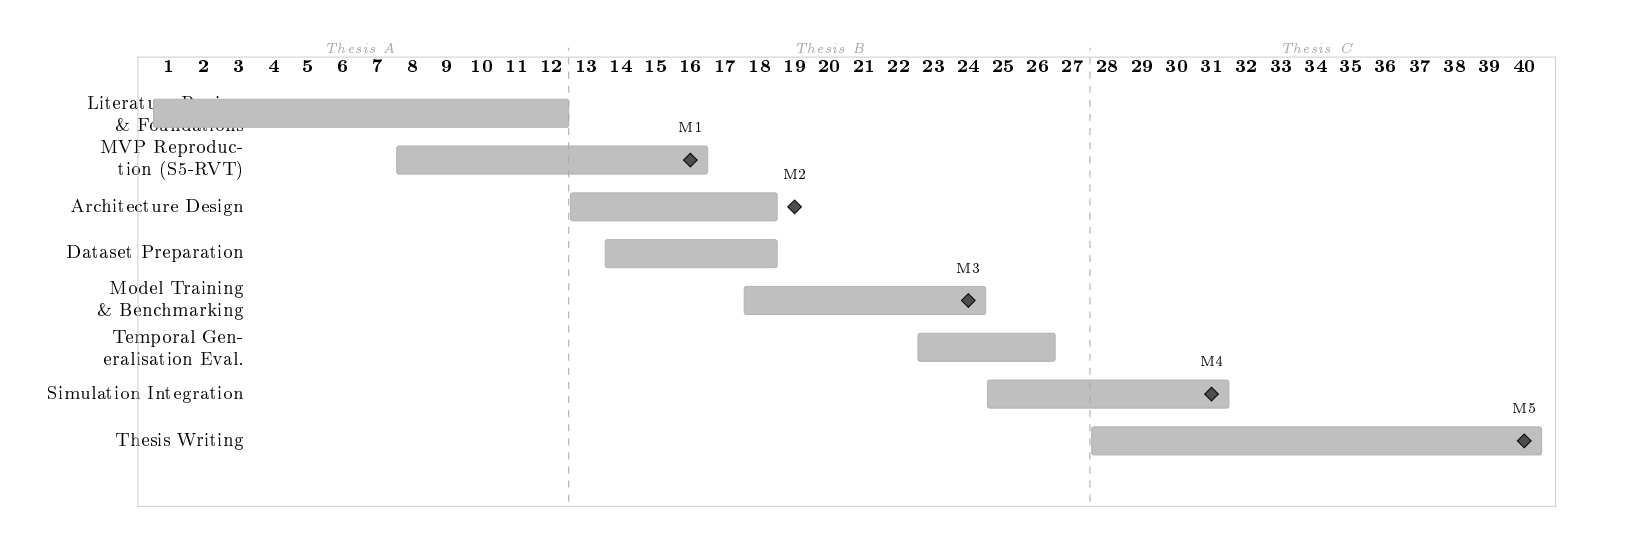
\includegraphics[width=\textwidth]{images/Ghantt Chart.png}
    \caption{Project Gantt chart showing the week-by-week schedule across all thesis phases. Thesis~A (Weeks 1--12) covers the literature review and MVP baseline reproduction. Thesis~B (Weeks 13--27) covers architecture design, dataset preparation, model training and benchmarking, temporal generalisation evaluation, and simulation integration. Thesis~C (Weeks 28--40) covers thesis writing and final submission. Diamond markers (M1--M5) indicate key milestone deliverables.}
    \label{fig:gantt}
\end{figure}

% --- Appendix B: Mathematical Formulations ---
\chapter{Mathematical Formulations}
\label{app:maths}

\section{Continuous-Time SSM}
A classical linear SSM evolves a latent state vector $h(t) \in \mathbb{R}^N$ according to a continuous-time linear dynamical system \cite{gu2022efficiently, gu2023mamba}:
\begin{align}
    h'(t) &= A h(t) + B u(t) \\
    y(t) &= C h(t) + D u(t)
\end{align}
where $u(t) \in \mathbb{R}$ is the scalar input, $y(t) \in \mathbb{R}$ is the scalar output, and $h(t) \in \mathbb{R}^N$ is the latent state. $A \in \mathbb{R}^{N \times N}$ is the state transition matrix, typically initialised via the HiPPO framework \cite{gu2022efficiently} to capture long-range history, while $B, C,$ and $D$ are learned projection matrices. The dimension $N$ controls the memory capacity of each SSM layer.

\section{Discretisation}
The continuous system is discretised at step size $\Delta$ using the zero-order hold (ZOH) method \cite{gu2023mamba}:
\begin{align}
    \overline{A} &= \exp(\Delta A) \\
    \overline{B} &= (\exp(\Delta A) - I) A^{-1} B
\end{align}
The resulting discrete recurrence is:
\begin{align}
    h_k &= \overline{A} h_{k-1} + \overline{B} u_k \\
    y_k &= C h_k + D u_k
\end{align}
This recurrence has time complexity $O(L \times N \times D)$ per layer for sequence length $L$, compared to the quadratic complexity $O(L^2 D)$ of self-attention.

\section{Mamba Selective Scan}
The selective SSM (Mamba \cite{gu2023mamba}) introduces input-dependency to the parameters $\Delta, B,$ and $C$:
\begin{equation}
    \Delta_k, B_k, C_k = f_\theta(u_k)
\end{equation}
where $f_\theta$ denotes learned linear projections. Input-dependent $\Delta_k$ enables selective retention: a large $\Delta_k$ causes rapid state decay (forgetting irrelevant content), while a small $\Delta_k$ preserves long-range memory.

\section{Voxel Grid Representation}
Event streams are converted to a $B$-bin voxel grid $V \in \mathbb{R}^{B \times H \times W}$. Each event $e_k = (x_k, y_k, t_k, p_k)$ contributes to bin $b$ via bilinear temporal interpolation \cite{zhu2019unsupervised}:
\begin{equation}
    V_b(x, y) = \sum_k p_k \cdot \max(0, 1 - |(B-1) \cdot t_k / T - b|) \cdot \delta(x-x_k) \cdot \delta(y-y_k)
\end{equation}
where $T$ is the total window duration, $B=10$ bins for the Gen1 dataset, and $\delta$ selects the matching pixel position. Each bin is independently normalised to zero mean and unit variance.

% --- Appendix C: Draft Thesis Outline ---
\chapter{Draft Thesis Outline}

\label{app:outline}

\noindent The following presents the planned chapter and section structure of the complete thesis document. Section headings are directly linked to the four research gaps identified in Chapter~2 and the experimental aims described in Chapter~3.

\bigskip

\noindent\textbf{1.\quad Introduction}\\[3pt]
\hspace*{2em}1.1\quad Background and Motivation\\[2pt]
\hspace*{2em}1.2\quad Problem Statement\\[2pt]
\hspace*{2em}1.3\quad Research Objectives\\[2pt]
\hspace*{2em}1.4\quad Thesis Contributions\\[2pt]
\hspace*{2em}1.5\quad Thesis Organisation

\bigskip

\noindent\textbf{2.\quad Literature Review}\\[3pt]
\hspace*{2em}2.1\quad Event-Based Cameras: Principles and Hardware\\[2pt]
\hspace*{2em}2.2\quad Event Representations for Deep Learning\\[2pt]
\hspace*{2em}2.3\quad Deep Learning for Event-Based Object Detection\\[2pt]
\hspace*{2em}2.4\quad State Space Models: Architecture and Evolution\\[2pt]
\hspace*{2em}2.5\quad State Space Models for Event Camera Data\\[2pt]
\hspace*{2em}2.6\quad Event-Based Vision for UAV Navigation\\[2pt]
\hspace*{2em}2.7\quad Research Gaps and Thesis Positioning

\bigskip

\noindent\textbf{3.\quad Methodology}\\[3pt]
\hspace*{2em}3.1\quad SSM-Based Detection Architecture Design\\[2pt]
\hspace*{2em}3.2\quad Event Representation Selection\\[2pt]
\hspace*{2em}3.3\quad Training Protocol and Hyperparameter Optimisation\\[2pt]
\hspace*{2em}3.4\quad Baseline Architectures for Comparison\\[2pt]
\hspace*{2em}3.5\quad Temporal Generalisation Evaluation Protocol\\[2pt]
\hspace*{2em}3.6\quad Obstacle Avoidance Integration Framework

\bigskip

\noindent\textbf{4.\quad Experimental Setup}\\[3pt]
\hspace*{2em}4.1\quad Datasets and Preprocessing\\[2pt]
\hspace*{2em}4.2\quad Evaluation Metrics\\[2pt]
\hspace*{2em}4.3\quad Hardware and Software Configuration\\[2pt]
\hspace*{2em}4.4\quad Simulation Environment

\bigskip

\noindent\textbf{5.\quad Results and Discussion}\\[3pt]
\hspace*{2em}5.1\quad Object Detection Performance\\[2pt]
\hspace*{2em}5.2\quad Computational Efficiency Analysis\\[2pt]
\hspace*{2em}5.3\quad Temporal Generalisation Results\\[2pt]
\hspace*{2em}5.4\quad Obstacle Avoidance Performance\\[2pt]
\hspace*{2em}5.5\quad Ablation Studies

\bigskip

\noindent\textbf{6.\quad Conclusion and Future Work}\\[3pt]
\hspace*{2em}6.1\quad Summary of Contributions\\[2pt]
\hspace*{2em}6.2\quad Limitations\\[2pt]
\hspace*{2em}6.3\quad Future Directions

\bigskip

\noindent\textbf{References}

\bigskip

\noindent\textbf{Appendices}

% --- Appendix D: Architectural Comparison ---
\chapter{Architectural Comparison}
\label{app:arch}

\begin{table}[h!]
    \centering
    \caption{Architectural comparison: CNN-SSM Hybrid vs. Pure SSM.}
    \label{tab:arch_comparison}
    \renewcommand{\arraystretch}{1.4}
    \begin{tabularx}{\textwidth}{|l|X|X|}
        \hline
        \rowcolor[gray]{0.9} \textbf{Dimension} & \textbf{CNN-SSM Hybrid (\textit{EventSSMDetector})} & \textbf{Pure SSM (\textit{PureSSMDetector})} \\ \hline
        Spatial extraction & ResNet-18 (stride-8 conv layers) & BiMamba over $16 \times 16$ patch tokens \\ \hline
        Temporal processing & Causal \texttt{MambaStack} & Causal \texttt{MambaStack} \\ \hline
        Spatial inductive bias & Strong --- local translation equivariance & Weak --- learned from data via 1D scan \\ \hline
        Est. parameter count & $\sim$8--9M & $\sim$4--5M \\ \hline
        CNN dependency & Yes & No --- fully SSM end-to-end \\ \hline
        Thesis role & Baseline with established spatial prior & Primary novel contribution \\ \hline
    \end{tabularx}
\end{table}

% --- Appendix E: Risk Assessment ---
\chapter{Risk Assessment}
\label{app:risk}

\begin{table}[h!]
    \centering
    \small
    \caption{Risk assessment for the thesis project.}
    \label{tab:risk_assessment}
    \renewcommand{\arraystretch}{1.5}
    \begin{tabularx}{\textwidth}{|>{\RaggedRight\arraybackslash}p{3cm}|l|l|>{\RaggedRight\arraybackslash}X|}
        \hline
        \rowcolor[gray]{0.9} \textbf{Risk} & \textbf{Likelihood} & \textbf{Impact} & \textbf{Mitigation} \\ \hline
        SSM model does not achieve competitive detection accuracy & Medium & High & Both a CNN-SSM hybrid and a pure SSM architecture have been implemented, enabling direct ablation. If the pure SSM underperforms, the hybrid serves as a fallback while still contributing an SSM-based comparison. \\ \hline
        Event camera hardware unavailable or delayed & Medium & Medium & Use publicly available datasets and simulation; focus on algorithmic contributions. \\ \hline
        Insufficient computational resources for training & Low & Medium & Leverage UNSW Katana cluster; use model distillation to reduce training cost. \\ \hline
        Obstacle avoidance integration proves infeasible within timeline & Medium & Medium & Prioritise detection benchmarking; use simulation-only evaluation if hardware integration delayed. \\ \hline
        Injury during physical UAV testing & Low & High & Conduct testing in designated flying areas with safety protocols; use protective equipment; obtain required certifications. \\ \hline
    \end{tabularx}
\end{table}

\addcontentsline{toc}{chapter}{References}
\bibliographystyle{ieeetr}
\bibliography{references}

\end{document}